% !TeX spellcheck = en_GB
\documentclass[12pt]{beamer}
\usepackage[utf8]{inputenc}
\usepackage[T1]{fontenc}
\usepackage{lmodern}
\usepackage[english]{babel}
\usepackage{amsmath}
\usepackage{amsfonts}
\usepackage{amssymb}
\usepackage{graphicx}
%\usetheme{Montpellier}
\newtheorem*{conjecture}{Conjecture}
\begin{document}
	\author{Paul Dubois}
	\title{Modular Forms Modulo 2:}
	\subtitle{Governing Fields for the Hecke Algebra}
	\logo{\includegraphics[scale=0.02]{ucl-logo.png}}
	\institute{University College of London}
	\date{March 25, 2020}
	\subject{Mathematics}
	%\setbeamercovered{transparent}
	%\setbeamertemplate{navigation symbols}{}
	\begin{frame}[plain]
		\maketitle
	\end{frame}
	
	\begin{frame}
		\frametitle{Modular Forms}
		\begin{center}
			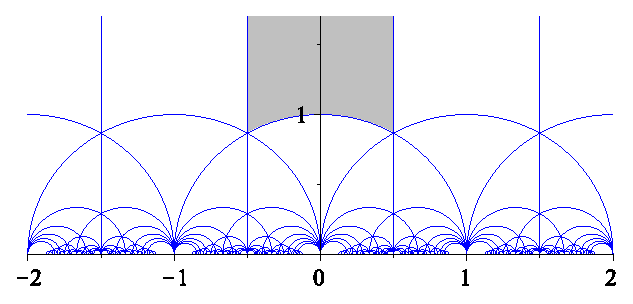
\includegraphics{ModularGroup-FundamentalDomain.eps}
		\end{center}
	\end{frame}

	\begin{frame}
		\frametitle{Reduction Modulo 2}
		$$M_n = \left\langle \Delta, E_2, E_2 \right\rangle$$
		
		$$\overline{\Delta} \rightsquigarrow \Delta$$
		$$\overline{E_2} \rightsquigarrow 1$$
		$$\overline{E_3} \rightsquigarrow 1$$
		
		$$\overline{M_n} \rightsquigarrow \left\langle \Delta \right\rangle$$
	\end{frame}

	\begin{frame}
		\frametitle{Modular Forms Modulo 2}
		$$
		\mathcal{F}
		= \left\langle \Delta^k \mid k \text{ odd} \right\rangle
		= \left\langle \Delta, \Delta^3, \Delta^5, \dots \right\rangle.
		$$
		\begin{align*}
			\Delta(q)
			&= q \prod_{n=1}^{\infty} (1-q^n)^{24}\\
			&= \sum_{n=0}^{\infty} \tau(n)q^n\\
			&\equiv \sum_{m=0}^{\infty} q^{(2m+1)^2} \bmod 2\\
		\end{align*}
	\end{frame}
	
%	\begin{frame}
%		\frametitle{Subspaces of Modular Forms Modulo 2}
%		$$
%		\mathcal{F}_1
%		= \left\langle \Delta^k \mid k = 1 \bmod 8 \right\rangle
%		= \left\langle \Delta^1, \Delta^9, \Delta^{17}, \Delta^{25}, \dots \right\rangle,
%		$$
%		$$
%		\mathcal{F}_3
%		= \left\langle \Delta^k \mid k = 3 \bmod 8 \right\rangle
%		= \left\langle \Delta^3, \Delta^{11}, \Delta^{19}, \Delta^{27}, \dots \right\rangle,
%		$$
%		$$
%		\mathcal{F}_5
%		= \left\langle \Delta^k \mid k = 5 \bmod 8 \right\rangle
%		= \left\langle \Delta^5, \Delta^{13}, \Delta^{21}, \Delta^{29}, \dots \right\rangle,
%		$$
%		$$
%		\mathcal{F}_7
%		= \left\langle \Delta^k \mid k = 7 \bmod 8 \right\rangle
%		= \left\langle \Delta^7, \Delta^{15}, \Delta^{23}, \Delta^{31}, \dots \right\rangle.
%		$$
%		$$
%		\mathcal{F} = \mathcal{F}_1 \oplus \mathcal{F}_3 \oplus \mathcal{F}_5 \oplus \mathcal{F}_7.
%		$$
%	\end{frame}
	
	\begin{frame}
		\frametitle{Hecke Operators}
		With
		$$
		f(q) = \sum_{n \in \mathbb{N}} c(n)q^n
		$$
		We define
		$$
		\overline{T_m}|f(q) = \sum_{n \in \mathbb{N}} \gamma(n)q^n
		$$
		Where
		$$
		\gamma(n) = \sum_{a | (n,m),\, a \geq 1} a^{2k-1} c\left( \frac{mn}{a^2} \right)
		$$
	\end{frame}
	\begin{frame}
		\frametitle{Hecke Operators Modulo 2}
		With
		$$
		f(q) = \sum_{n \in \mathbb{N}} c(n)q^n
		$$
		We define
		$$
		\overline{T_p}|f(q) = \sum_{n \in \mathbb{N}} \gamma(n)q^n
		$$
		Where
		$$
		\gamma(n) = 
		\left\lbrace
		\begin{array}{l l}
		c(np)        & \text{ if } p \nmid n \\
		c(np)+c(n/p) & \text{ if } p \mid  n
		\end{array}
		\right. 
		\quad \text{ and } p \text{ an odd prime}.
		$$
	\end{frame}

	\begin{frame}
		\frametitle{Examples}
		$$T_{11}\Delta^{29}$$
		[a few more examples]
	\end{frame}

	\begin{frame}
		\frametitle{The Hecke Algebra}
		$$
		A
		= \left\langle T_3, T_5, T_7, T_{11}, T_{13}, \dots  \right\rangle
		= \left\langle T_p \mid p \in \mathbb{P} \right\rangle
		$$
		
		$$A = \mathbb{F}_2 \left[\left[ T_3, T_5 \right]\right]$$
		
		$$T_p = \sum_{i+j \geq 1} a_{ij}(p) T_3^iT_5^j$$
	\end{frame}

	\begin{frame}
		\frametitle{Example}
		$$T_{19}$$
		[a few examples]
	\end{frame}

	\begin{frame}
		\frametitle{Dirichlet Density Theorem: Intuition}
		\boxed{\href{https://pauldubois98.github.io/DirichletDensityTheoremAnimation/}{Animation}}
		(see \url{https://pauldubois98.github.io/DirichletDensityTheoremAnimation/})
	\end{frame}
	\begin{frame}
		\frametitle{Dirichlet Density Theorems}
		[to write]
	\end{frame}
	
	\begin{frame}
		\frametitle{Frobenius element}
		[define frob elements quickly]
	\end{frame}
	\begin{frame}
		\frametitle{Chebotarev Density Theorems}
		[to write]
	\end{frame}

	\begin{frame}
		\frametitle{Frobenian Maps}
		[definition]
	\end{frame}
	\begin{frame}
		\frametitle{The maps $a_{ij}$}
		$$T_p = \sum_{i+j \geq 1} a_{ij}(p) T_3^iT_5^j$$
		\vspace{1cm}
		$$a_{ij}: p \mapsto a_{ij}(p)$$
	\end{frame}
	\begin{frame}
		\frametitle{Known Governing Fields}
		$$M_{01} = \mathbb{Q}\left(\zeta_8\right)$$
		$$M_{02} = \mathbb{Q}\left(\zeta_8, \sqrt[4]{2}\right)$$
	\end{frame}
	\begin{frame}
		\frametitle{Potential New Governing Fields}
		$$M_{03} \stackrel{?}{=} \mathbb{Q}\left(\zeta_8, \sqrt[4]{2}, \sqrt{\alpha}\right)$$
		where:
		\begin{align*}
			\alpha =
			&- \frac{3136435454775881 \sqrt[4]{2}}{562949953421312} + \frac{4208721080340285 \sqrt{2}}{2251799813685248} +\\
			&\frac{3672578267558083 \cdot \sqrt[4]{2}^3}{562949953421312} + \frac{3582104167901087}{281474976710656}
		\end{align*}
	\end{frame}
	\begin{frame}
	\frametitle{Potential New Governing Fields}
		$$M_{05} \stackrel{?}{=}\mathbb{Q}\left(\zeta_8, \sqrt[4]{2}, \sqrt{\alpha}, \sqrt{\beta}\right)$$
		where:
		\begin{align*}
			\alpha =
			&- \frac{3136435454775881 \sqrt[4]{2}}{562949953421312} + \frac{4208721080340285 \sqrt{2}}{2251799813685248} \\
			&+ \frac{3672578267558083 \cdot \sqrt[4]{2}^3}{562949953421312} + \frac{3582104167901087}{281474976710656}
		\end{align*}
		and
		\begin{align*}
		\beta = 
		&- \frac{8282936156772053 \alpha^{\frac{13}{2}}}{1125899906842624} 
		- \frac{1240182980093567 \alpha^{6}}{562949953421312} \\
		&- \frac{336382584949535 \alpha^{\frac{9}{2}}}{2199023255552} 
		- \frac{6445823996745319 \alpha^{4}}{140737488355328} \\
		&-\dots \\
%		&- \frac{4638634719581101 \alpha^{\frac{5}{2}}}{35184372088832} 
%		- \frac{2954723016803317 \alpha^{2}}{70368744177664} 
%		\\
%		&- \frac{5142889464378747 \sqrt[4]{2}}{140737488355328} 
%		- \frac{4198844765367981 \sqrt{\alpha}}{1125899906842624} \\
%		&+ \frac{3450571136356681 \sqrt{2}}{281474976710656} 
%		+ \frac{6022015868546055 \cdot \sqrt[4]{2}^3}{140737488355328} \\
%		&+ \frac{5763554133419461}{70368744177664} 
%		+ \frac{7633450872164841 \alpha^{\frac{3}{2}}}{281474976710656} 
%		\\
%		&+ \frac{615248862392953 \alpha^{3}}{8796093022208} 
%		+ \frac{8240373942248553 \alpha^{\frac{7}{2}}}{35184372088832} \\
%		&+ \frac{8030384673908857 \alpha^{5}}{562949953421312} 
%		+ \frac{4981425151744809 \alpha^{7}}{18014398509481984} \\
%		&+ \frac{1676680829315919 \alpha^{\frac{11}{2}}}{35184372088832} 
%		+ \frac{8299866982438859 \alpha^{\frac{15}{2}}}{9007199254740992}
		\end{align*}
	\end{frame}
	
	\begin{frame}
		\frametitle{Governing Groups}
		$$G_{01} = D_{8} \qquad G_{10} = D_{8}$$
		$$G_{02} = D_{8} \qquad G_{20} = D_{8}$$
		$$G_{03} = D_{16} \qquad G_{30} = D_{16}$$
		$$G_{04} = D_{16} \qquad G_{40} = D_{16}$$
		$$G_{05} = D_{32} \qquad G_{50} = D_{32}$$
		$$G_{06} = D_{32} \qquad G_{60} = D_{32}$$
		$$G_{07} = D_{32} \qquad G_{70} = D_{32}$$
	\end{frame}

	\begin{frame}
		\frametitle{Diagonal Governing Groups}
		\begin{conjecture}[Diagonal Governing Groups Conjecture]
			For all $k \in \mathbb{N}^*$, there exists a field $M_{0k}$ such that $M_{0k}$ is a governing field for $a_{0k}$, and $G_{0k} = \text{Gal}(M_{0k}/\mathbb{Q})$ is dihedral.\\
			For all $k \in \mathbb{N}^*$, there exists a field $M_{k0}$ such that $M_{k0}$ is a governing field for $a_{k0}$, and $G_{k0}$ is dihedral.\\
			\ \\
			Moreover $M_{k0} \neq M_{0k}$ in general, but $G_{k0} \cong G_{0k}$.
		\end{conjecture}
	\end{frame}

	\begin{frame}
		\frametitle{Questions}
		[add some usefull links?]
	\end{frame}
	

\end{document}